\documentclass{beamer}
\usepackage[utf8]{inputenc}

\usetheme{Madrid}
\usecolortheme{default}
\usepackage{amsmath,amssymb,amsfonts,amsthm}
\usepackage{txfonts}
\usepackage{tkz-euclide}
\usepackage{listings}
\usepackage{adjustbox}
\usepackage{array}
\usepackage{tabularx}
\usepackage{gvv}
\usepackage{lmodern}
\usepackage{circuitikz}
\usepackage{tikz}
\usepackage{graphicx}
\usepackage{mathtools}

\setbeamertemplate{page number in head/foot}[totalframenumber]

\usepackage{tcolorbox}
\tcbuselibrary{minted,breakable,xparse,skins}



\definecolor{bg}{gray}{0.95}
\DeclareTCBListing{mintedbox}{O{}m!O{}}{%
  breakable=true,
  listing engine=minted,
  listing only,
  minted language=#2,
  minted style=default,
  minted options={%
    linenos,
    gobble=0,
    breaklines=true,
    breakafter=,,
    fontsize=\small,
    numbersep=8pt,
    #1},
  boxsep=0pt,
  left skip=0pt,
  right skip=0pt,
  left=25pt,
  right=0pt,
  top=3pt,
  bottom=3pt,
  arc=5pt,
  leftrule=0pt,
  rightrule=0pt,
  bottomrule=2pt,
  toprule=2pt,
  colback=bg,
  colframe=orange!70,
  enhanced,
  overlay={%
    \begin{tcbclipinterior}
    \fill[orange!20!white] (frame.south west) rectangle ([xshift=20pt]frame.north west);
    \end{tcbclipinterior}},
  #3,
}
\lstset{
    language=C,
    basicstyle=\ttfamily\small,
    keywordstyle=\color{blue},
    stringstyle=\color{orange},
    commentstyle=\color{green!60!black},
    numbers=left,
    numberstyle=\tiny\color{gray},
    breaklines=true,
    showstringspaces=false,
}
\title{10.6.1}
\date{1st October, 2025}
\author{Puni Aditya - EE25BTECH11046}

\begin{document}

\frame{\titlepage}
\begin{frame}{Question}
Draw a circle of radius 2.5cm. Take a point P outside the circle at a distance of 7cm from the center. Then construct a pair of tangents to the circle from point P.
\end{frame}

\begin{frame}{Theoretical Solution}
The tangent directions $\vec{m}$ from an external point $\vec{h}$ to the circle $g\brak{\vec{x}}=\vec{x}^\top\vec{x}-r^2=0$ satisfy $\vec{m}^\top\vec{\Sigma}\vec{m} = 0$, where
\begin{align}
    \vec{\Sigma} = \vec{h}\vec{h}^\top - g\brak{\vec{h}}\vec{I} \label{eq:sigma_def}
\end{align}
With the point $\vec{h}=d\vec{e_1}$, we have $g\brak{\vec{h}} = d^2-r^2$. From \eqref{eq:sigma_def},
\begin{align}
    \vec{\Sigma} &= \myvec{d^2 & 0 \\ 0 & 0} - \myvec{d^2-r^2 & 0 \\ 0 & d^2-r^2} \nonumber \\
    &= \myvec{r^2 & 0 \\ 0 & -\brak{d^2-r^2}}
\end{align}
\end{frame}

\begin{frame}{Theoretical Solution}
Since $\vec{\Sigma}$ is a diagonal matrix, its eigenvalues are the diagonal entries.
\begin{align}
 \lambda_1 = r^2, \text{ } \lambda_2 = -\brak{d^2-r^2}
\end{align}
The matrix of orthonormal eigenvectors is 
\begin{align}
	\vec{P}=\vec{I}
\end{align}
The unit direction vectors of the tangents are given by the formula:
\begin{align}
    \vec{m} = \frac{1}{\sqrt{\lambda_1-\lambda_2}}\vec{P}\myvec{\sqrt{-\lambda_2} \\ \pm\sqrt{\lambda_1}} \label{eq:m_formula}
\end{align}
\end{frame}

\begin{frame}{Theoretical Solution}
We calculate the terms for \eqref{eq:m_formula}:
\begin{align}
    \lambda_1-\lambda_2 &= r^2 - \brak{-\brak{d^2-r^2}} = d^2 \\
    -\lambda_2 &= d^2-r^2
\end{align}
Substituting these into \eqref{eq:m_formula}:
\begin{align}
    \vec{m} &= \frac{1}{\sqrt{d^2}}\vec{I}\myvec{\sqrt{d^2-r^2} \\ \pm\sqrt{r^2}} = \frac{1}{d}\myvec{\sqrt{d^2-r^2} \\ \pm r}
\end{align}
\end{frame}

\begin{frame}{Theoretical Solution}
The points of contact are $\vec{q} = \vec{h} + \kappa\vec{m}$. The parameter $\kappa$ is found by substituting the line equation into the circle equation:
\begin{align}
    g\brak{\vec{h}+\kappa\vec{m}} = \brak{\vec{h}+\kappa\vec{m}}^\top\brak{\vec{h}+\kappa\vec{m}} - r^2 = 0 \\
    \kappa^2\brak{\vec{m}^\top\vec{m}} + 2\kappa\brak{\vec{h}^\top\vec{m}} + g\brak{\vec{h}} = 0
\end{align}
For a tangent, this quadratic has a single repeated root.
\end{frame}

\begin{frame}{Theoretical Solution}
Since $\vec{m}$ is a unit vector, the value of $\kappa$ for the point of contact is:
\begin{align}
    \kappa = \frac{-2\brak{\vec{h}^\top\vec{m}}}{2\brak{1}} = -\vec{h}^\top\vec{m}
\end{align}
We require $\kappa<0$, which implies $\vec{h}^\top\vec{m}>0$.
\begin{align}
    \vec{h}^\top\vec{m} = \brak{d\vec{e_1}}^\top\frac{1}{d}\myvec{\sqrt{d^2-r^2} \\ \pm r} = \sqrt{d^2-r^2} > 0
\end{align}
The condition is satisfied, and so $\kappa = -\sqrt{d^2-r^2}$.
\end{frame}

\begin{frame}{Theoretical Solution}
The points of contact are $\vec{q} = \vec{h} + \kappa\vec{m}$.
\begin{align}
    \vec{q} &= d\vec{e_1} - \sqrt{d^2-r^2}\brak{\frac{1}{d}\myvec{\sqrt{d^2-r^2} \\ \pm r}} \nonumber \\
    &= \myvec{d \\ 0} - \myvec{\frac{d^2-r^2}{d} \\ \pm \frac{r\sqrt{d^2-r^2}}{d}} \nonumber \\
    &= \myvec{\frac{r^2}{d} \\ \mp \frac{r\sqrt{d^2-r^2}}{d}}
\end{align}
\end{frame}

\begin{frame}{Final Calculation}
Substituting $r=2.5$ and $d=7$:
\begin{align}
    \vec{q} &= \myvec{\frac{\brak{2.5}^2}{7} \\ \pm\frac{2.5\sqrt{7^2 - \brak{2.5}^2}}{7}} \nonumber \\
    &= \myvec{\frac{6.25}{7} \\ \pm\frac{2.5\sqrt{42.75}}{7}} = \myvec{\frac{25}{28} \\ \pm\frac{2.5\sqrt{42.75}}{7}}
\end{align}
\end{frame}

\begin{frame}{Plot}
\begin{figure}
    \centering
    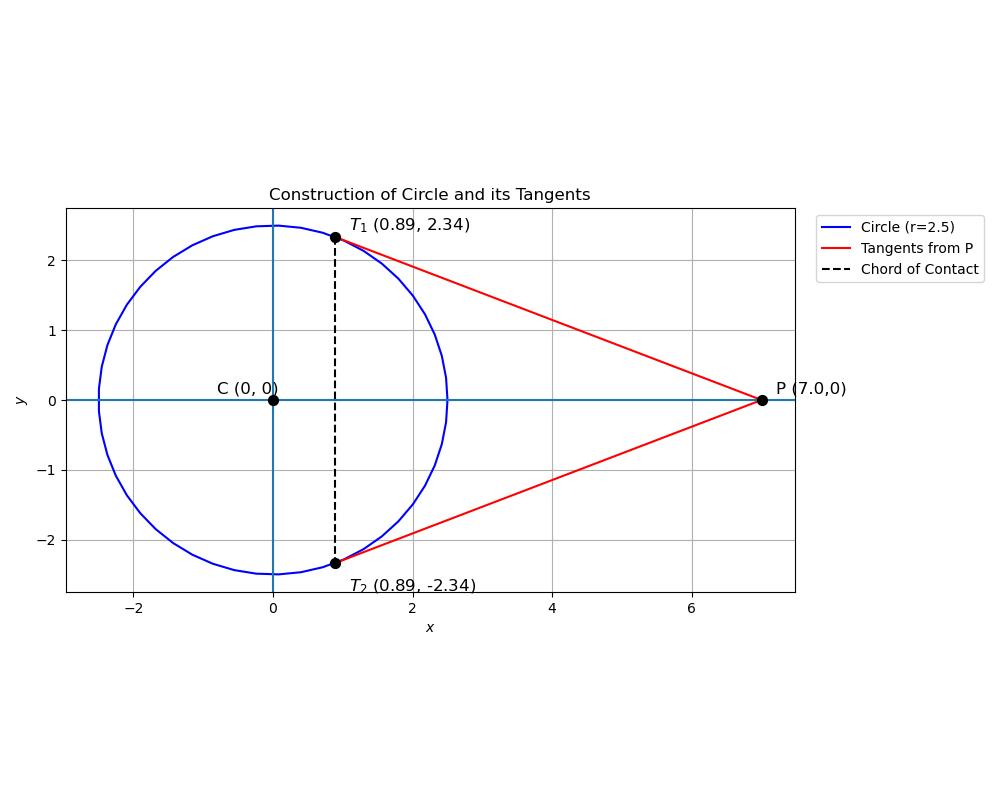
\includegraphics[width=0.5\columnwidth]{../figs/plot_c.jpg}
    \caption{Plot}
    \label{fig:fig}
\end{figure}
\end{frame}

\end{document}
